\documentclass[a4paper,10pt,twocolumn]{ltjarticle}
\usepackage{kaitoushu}

\pgfplotsset{
  myaxis/.style={
    axis lines=middle,
    xlabel={$x$}, ylabel={$y$},
    every axis x label/.style={at={(ticklabel* cs:1)},anchor=west},
    every axis y label/.style={at={(ticklabel* cs:1)},anchor=south},
    tick label style={font=\scriptsize},
    label style={font=\small},
    width=5.5cm, height=5cm,
    grid=none,
    samples=200,
  }
}

\begin{document}

\problemrange{3章：関数とグラフ — 練習問題2・A (p.99)}



\mondai{1}{次の関数について，奇関数か偶関数かを調べよ．}
\kotae{
$f(-x)=f(x)$ なら偶関数，$f(-x)=-f(x)$ なら奇関数．

(1) $y=\dfrac{x^{2}}{\sqrt{x^{2}+1}}$

$f(-x)=\dfrac{(-x)^{2}}{\sqrt{(-x)^{2}+1}}=\dfrac{x^{2}}{\sqrt{x^{2}+1}}=f(x)$ → \textbf{偶関数}

(2) $y=x^{5}-3x^{3}$

$f(-x)=-x^{5}+3x^{3}=-(x^{5}-3x^{3})=-f(x)$ → \textbf{奇関数}

(3) $y=x^{6}+3x^{3}$

$f(-x)=x^{6}-3x^{3}$．$f(x)$ とも $-f(x)$ とも一致しない．→ \textbf{どちらでもない}

(4) $y=|x|+1$

$f(-x)=|-x|+1=|x|+1=f(x)$ → \textbf{偶関数}
}

\mondai{2}{次の関数のグラフをかけ．}
\kotae{
(1) $y=(x+1)^{3}+2$：$y=x^{3}$ を $x$ 方向に $-1$，$y$ 方向に $2$ 平行移動．変曲点 $(-1,2)$．

\begin{tikzpicture}
\begin{axis}[myaxis, xmin=-3,xmax=1,ymin=-3,ymax=7]
\addplot[thick,blue,domain=-2.5:0.5]{(x+1)^3+2};
\addplot[only marks,mark=*,mark size=1.5pt] coordinates {(-1,2)};
\end{axis}
\end{tikzpicture}

(2) $y=-(x-2)^{4}+1$：上に凸，最大 $(2,1)$．

\begin{tikzpicture}
\begin{axis}[myaxis, xmin=0,xmax=4,ymin=-5,ymax=2]
\addplot[thick,blue,domain=0.7:3.3]{-(x-2)^4+1};
\addplot[only marks,mark=*,mark size=1.5pt] coordinates {(2,1)};
\end{axis}
\end{tikzpicture}

(3) $y=\dfrac{x}{x-1}=1+\dfrac{1}{x-1}$：漸近線 $x=1,\;y=1$

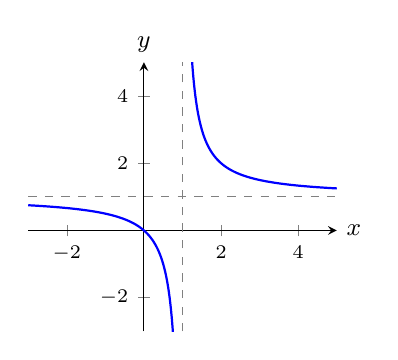
\begin{tikzpicture}
\begin{axis}[myaxis, xmin=-3,xmax=5,ymin=-3,ymax=5]
\addplot[thick,blue,domain=-3:0.8]{x/(x-1)};
\addplot[thick,blue,domain=1.2:5]{x/(x-1)};
\addplot[dashed,gray] coordinates {(1,-3)(1,5)};
\addplot[dashed,gray] coordinates {(-3,1)(5,1)};
\end{axis}
\end{tikzpicture}

(4) $y=\dfrac{2-x}{x+1}=-1+\dfrac{3}{x+1}$：漸近線 $x=-1,\;y=-1$

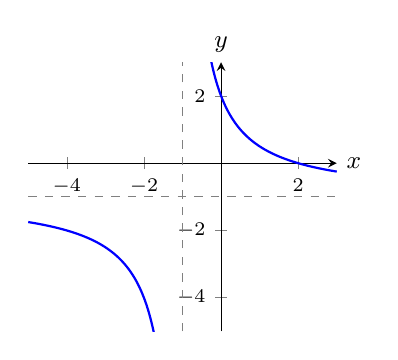
\begin{tikzpicture}
\begin{axis}[myaxis, xmin=-5,xmax=3,ymin=-5,ymax=3]
\addplot[thick,blue,domain=-5:-1.2]{(2-x)/(x+1)};
\addplot[thick,blue,domain=-0.8:3]{(2-x)/(x+1)};
\addplot[dashed,gray] coordinates {(-1,-5)(-1,3)};
\addplot[dashed,gray] coordinates {(-5,-1)(3,-1)};
\end{axis}
\end{tikzpicture}

(5) $y=\sqrt{x+4}-2$：$y=\sqrt{x}$ を $x$ 方向に $-4$，$y$ 方向に $-2$．始点 $(-4,-2)$．

\begin{tikzpicture}
\begin{axis}[myaxis, xmin=-5,xmax=5,ymin=-3,ymax=2]
\addplot[thick,blue,domain=-4:5]{sqrt(x+4)-2};
\addplot[only marks,mark=*,mark size=1.5pt] coordinates {(-4,-2)};
\end{axis}
\end{tikzpicture}

(6) $y=-\sqrt{2-x}+3$：定義域 $x\leqq2$．始点 $(2,3)$．

\begin{tikzpicture}
\begin{axis}[myaxis, xmin=-5,xmax=3,ymin=-1,ymax=4]
\addplot[thick,blue,domain=-5:2]{-sqrt(2-x)+3};
\addplot[only marks,mark=*,mark size=1.5pt] coordinates {(2,3)};
\end{axis}
\end{tikzpicture}
}

\mondai{3}{定義域が $0\leqq x\leqq 3$ である関数 $y=\dfrac{x-3}{x+1}$ の値域を求めよ．}
\kotae{
$y=\dfrac{x-3}{x+1}=\dfrac{(x+1)-4}{x+1}=1-\dfrac{4}{x+1}$

$x+1>0$ で $x$ が増加すると $\dfrac{4}{x+1}$ は減少，よって $y$ は単調増加．

$x=0$：$y=-3$\quad $x=3$：$y=0$

$\therefore -3\leqq y\leqq 0$
}

\mondai{4}{関数 $y=\dfrac{ax+b}{x+2}$ のグラフが点 $(-1,3)$ を通り，1つの漸近線が $y=2$ であるとき，定数 $a$，$b$ の値を定めよ．}
\kotae{
分子を整理：
\[
\dfrac{ax+b}{x+2}=\dfrac{a(x+2)+(b-2a)}{x+2}=a+\dfrac{b-2a}{x+2}
\]

漸近線 $y=a=2$ より $a=2$．

点 $(-1,3)$ 代入：$\dfrac{-2+b}{1}=3 \Rightarrow b=5$

$\therefore a=2,\;b=5$
}

\mondai{5}{関数 $y=\sqrt{x-3}\;(3\leqq x\leqq a)$ の値域が $0\leqq y\leqq 3$ であるとき，定数 $a$ の値を定めよ．}
\kotae{
$y=\sqrt{x-3}$ は単調増加．$x=3$：$y=0$．

$y=3$ のとき：$\sqrt{x-3}=3 \Rightarrow x-3=9 \Rightarrow x=12$

$\therefore a=12$
}

\mondai{6}{次の関数の逆関数を求めよ．}
\kotae{
$y=f(x)$ を $x$ について解き，$x$ と $y$ を入れ替える．

(1) $y=-ax+b\;(a\neq0)$

$ax=b-y \Rightarrow x=\dfrac{b-y}{a}$

$\therefore y=\dfrac{b-x}{a}\;\left(=-\dfrac{x}{a}+\dfrac{b}{a}\right)$

(2) $y=1-x^{2}\;(x\leqq0)$

$x^{2}=1-y$．$x\leqq0$ なので $x=-\sqrt{1-y}$．

$\therefore y=-\sqrt{1-x}\;(x\leqq1)$

(3) $y=\dfrac{a}{x-b}\;(a\neq0)$

$x-b=\dfrac{a}{y} \Rightarrow x=\dfrac{a}{y}+b$

$\therefore y=\dfrac{a}{x}+b$

(4) $y=\dfrac{x-3}{x+2}$

$y(x+2)=x-3 \Rightarrow x(y-1)=-2y-3$
\[
x=\dfrac{-2y-3}{y-1}=\dfrac{2y+3}{1-y}
\]

$\therefore y=\dfrac{2x+3}{1-x}$
}

\mondai{7}{関数 $y=(x-2)^{2}+3\;(x\geqq2)$ の逆関数を求めよ．また，もとの関数と逆関数のグラフをかけ．}
\kotae{
$x\geqq2$ より $x-2\geqq0$．

$(x-2)^{2}=y-3 \Rightarrow x-2=\sqrt{y-3} \Rightarrow x=2+\sqrt{y-3}$

$\therefore$ 逆関数 $y=2+\sqrt{x-3}\;(x\geqq3)$

両者は直線 $y=x$ に関して対称：

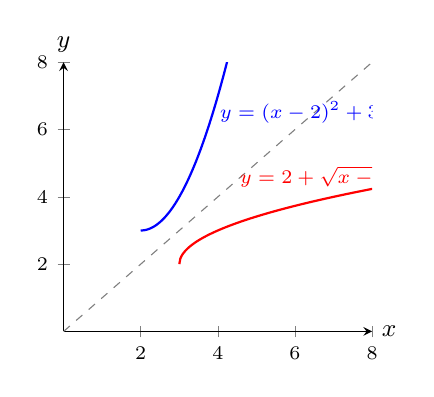
\begin{tikzpicture}
\begin{axis}[myaxis, xmin=0,xmax=8,ymin=0,ymax=8]
\addplot[thick,blue,domain=2:4.3]{(x-2)^2+3};
\addplot[thick,red,domain=3:8]{2+sqrt(x-3)};
\addplot[dashed,gray,domain=0:8]{x};
\node[blue,font=\scriptsize,right] at (axis cs:3.8,6.5) {$y=(x-2)^2+3$};
\node[red,font=\scriptsize,above] at (axis cs:6.5,4) {$y=2+\sqrt{x-3}$};
\end{axis}
\end{tikzpicture}
}

\end{document}
